Face detection and recognition is not a new subject to computer science. Through time there were many attempts to provide satisfactory solution and approximation. Techniques used for face detection spans from a regular well-known image recognition via edge detection, to more advanced, precise, though computationally expensive use of neural networks. This chapter will provide a basic overview of the mainstream approaches, listing the most current state-of-the-art methods and means to the problem.

Each section in this chapter represents a family of solutions. Providing a full description, explanation and understanding of their respective problem would span a book of its own, hence we aim to cover only a high level walk-though. We may also revisit certain aspects in more detail later in the text, as well.

\section{Convolutional neural networks}

There are many kinds of neural networks, one of which is called Convolutional Network\,\cite[p.~330]{deeplearningbook}, or CNN (Convolutional Neural Network). CNN specialises in processing data of known, grid-like structure. That includes for example time-series data, which can be represented as one dimensional grid of samples taken in regular intervals during period of time. It also includes image data, represented as 2D grid of pixels. As the name suggests, CNNs employs a mathematical operation called \textbf{convolution}. In practical application, that stands for a substitution of a matrix multiplication by this linear mathematical operation - convolution. And this is done in at least one of the network's layers.

This section aims to explain what convolution is, what are the motivations behind its usage in neural networks. Later we'll describe a \textbf{pooling} operation, which is used in almost all CNNs as well.

\subsection{Convolution}
\label{ss:conv}

Convolution as a mathematical operation generally symbolise an operation on two functions of real-valued argument. Let's start with an example, paraphrased from Hinton's book\,\cite{deeplearningbook}. of such functions and demonstrate a motivation behind convolution:

Assume we have a vehicle and a laser parking sensor mounted on its front. This sensor is used to measures a distance to some object, let's say a docking station for the vehicle. And we want to park the vehicle at some precise proximity to the object. The sensor provides a single output $p(t)$, which reads as a position of the vehicle at certain time. Both $p$ and $t$ are real-valued, which means that the sensor can provide a different output value at any instance in time.

We also have to count in that our sensor is not always fully precise and reliable, so the measurements provided may be noisy. To obtain a more relevant data\,--\,a less noisy estimate of the position against the object, we can base our measurement on an average of several data samples. Since the vehicle is moving, we have to assume that more recent outputs should provide more relevant reading. So, we can weight our average and give the more recent data points more importance. Let's define this weight function as $w(a)$, where the argument $a$ symbolize age of a measurement.

Calculating the weighted average at every moment, we can get a smoother estimation of the vehicle's position as a new function:

\begin{equation}
    s(t) = \int p(a) w(t - a) da
\end{equation}


The function $s$ is formally known as \textbf{convolution}. An asterisk symbol is usually used to denote this operation:

\begin{equation}
    s(t) = (p * w)(t)
\end{equation}

To complete the definition, we have to note that $w$ has to be a valid probability density function, which in our example has to meet a criteria $a < 0: w(a) = 0$. That limits our function to weight only past samples, since we can's assume that our sensor can look into the future, that would be silly. That is a limitation to our use case only. In general, convolution is defined for all functions where the integral above is defined.

Convolutional neural networks use a bit different terminology, than we used in the example. The function providing data we want to consume ($p$ from the example) is simply called \textbf{input}. The other parameter to the convolution, in our example that was the weight function, is called a \textbf{kernel}. The result of convolution ($s$) of input ($p$) over a kernel ($w$) is simply called \textbf{output} or \textbf{feature map}.

Our expectation that the sensor from the example above, would provide a measurement continuously, in any instant of time, is not realistic. Time is usually discretized in digital world, therefore it is meaningful to assume the sensor is providing measurements at regular intervals. So instead of integrating over time continuum, we can define a discrete convolution as:

\begin{equation}
    s(t) = \sum_{a=-\infty}^{\infty} p(a) w(t - a) = (p * w)(t)
\end{equation}

Our example was quite simple and straightforward, usually in artificial intelligence and deep-learning the input is common to be multidimensional array (tensor) of data. Also the kernel happens to be a tensor of parameters which values are often obtained by some learning algorithm.

Finally, when processing multidimensional data, convolution is used over multiple axis at the same time. That's important for our application, because pictures, we are about to process, have more than one dimension. So in case we have an input image $I$\,--\,a two-dimensional bitmap, our convolution should use a two-dimensional kernel $K$ as well:

\begin{equation}
    S(x,y) = (I * K)(x, y) = \sum_i\sum_j I(m, n) K(x - i)(y - j)
\end{equation}

\begin{figure}[ht]
    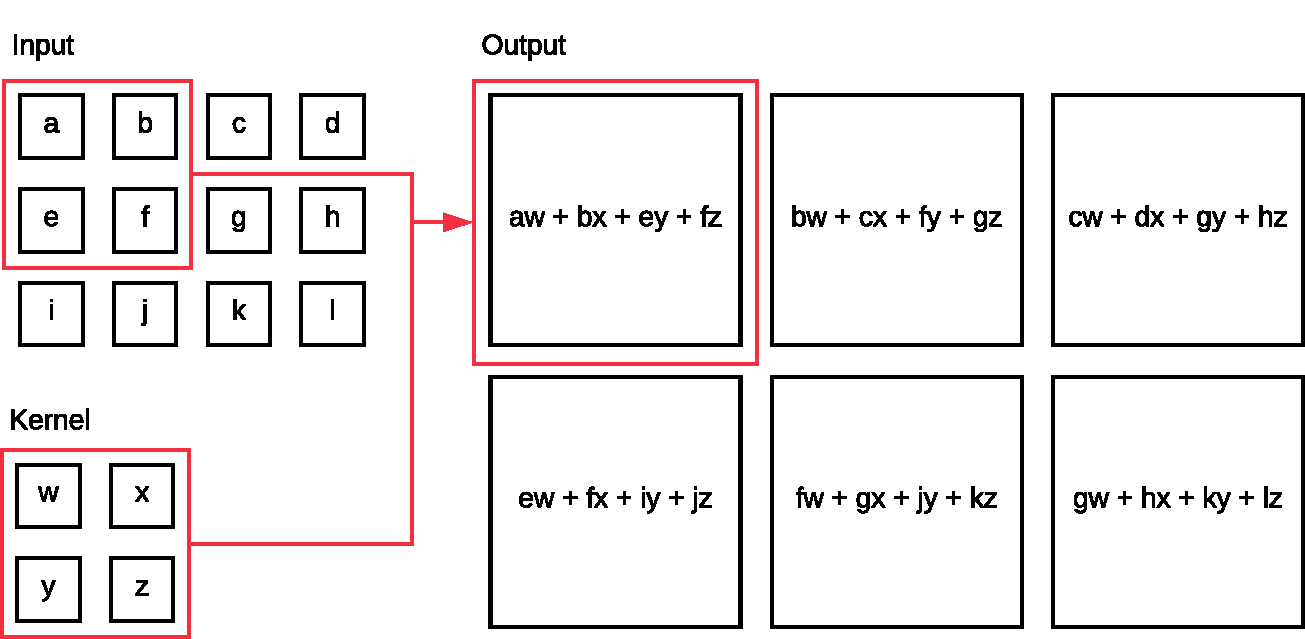
\includegraphics[width=\textwidth]{obrazky-figures/convolution.pdf}
    \caption{Convolution operation with 2D input data and 2D kernel}\label{fig:convolution}
\end{figure}

\subsection{Use of convolution in neural networks}

In machine learning, we leverage multiple important properties of the convolution operation:

\begin{itemize}
    \item Sparse interaction
    \item Sharing of parameters
    \item Equivariant representation
    \item Input of variable size
\end{itemize}

\subsubsection{Sparse interaction}

As you can notice in figure\,\ref{fig:convolution}, kernel can be of different size than input. When the input data is for example an image of millions of pixels, the size of kernel allows convolution to select only specific subset of inputs for each output. In traditional neural networks, a matrix multiplication is used instead of convolution. That means every output unit interacts with every input unit. In convolutional networks, the kernel size limits that just to certain subset of input units. It is called \textbf{sparse interaction}\,\cite[p.~335]{deeplearningbook} or \textbf{sparse weights} and it is accomplished by restricting kernel to a smaller size than the input. That results in smaller memory footprint of the model, since it requires fewer parameters to be stored. while at the same time it improves statistical efficiency. It has also impact on performance, since computing the output requires fewer operations compared to matrix multiplication. A graphical demonstration can be seen on figure\,\ref{fig:sparse_b}.

\begin{figure}[ht]
    \centering
    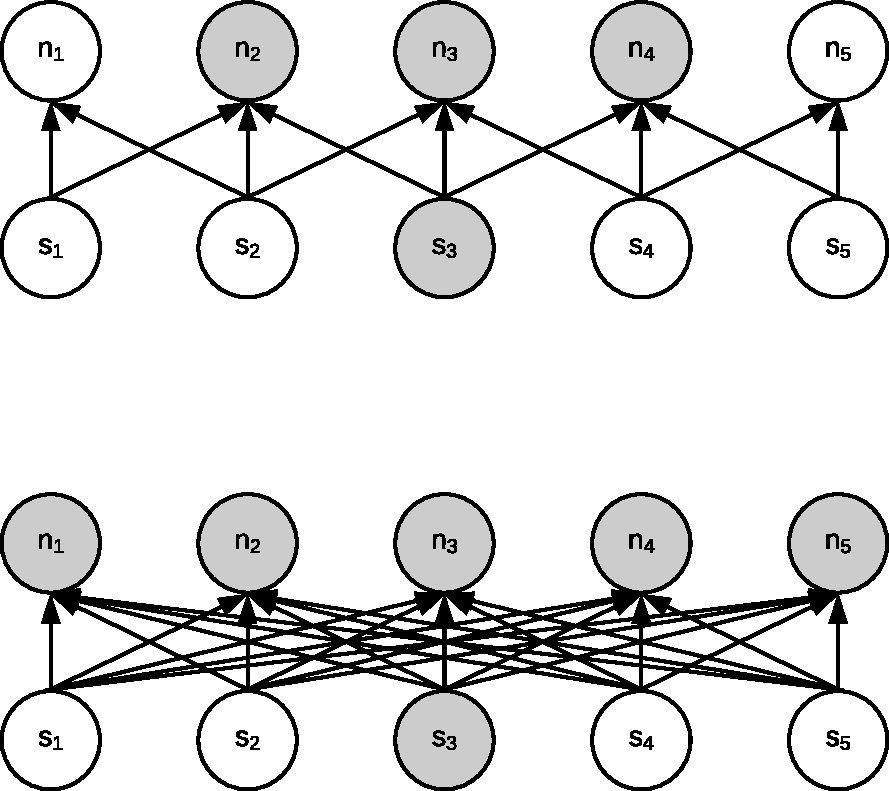
\includegraphics[width=.6\textwidth]{obrazky-figures/sparse_b.pdf}
    \caption{\textit{Sparse interaction viewed from below}: The highlighted units demonstrates propagation of one input unit from current layer $s_3$ to the next layer. On the top you can see all the output $n$ units, which are affected by this particular input. On the bottom picture, you can see how the same situation is represented in traditional matrix multiplication.}\label{fig:sparse_b}
\end{figure}

Deep convolutional networks allow indirect interaction between units which would be out of reach for given kernel size. This property is called \textbf{receptive field}\,\cite[p.~337]{deeplearningbook} of a unit and can be seen when we look at the network from perspective of the output layer (see figure\,\ref{fig:sparse_a}).

\begin{figure}[ht]
    \centering
    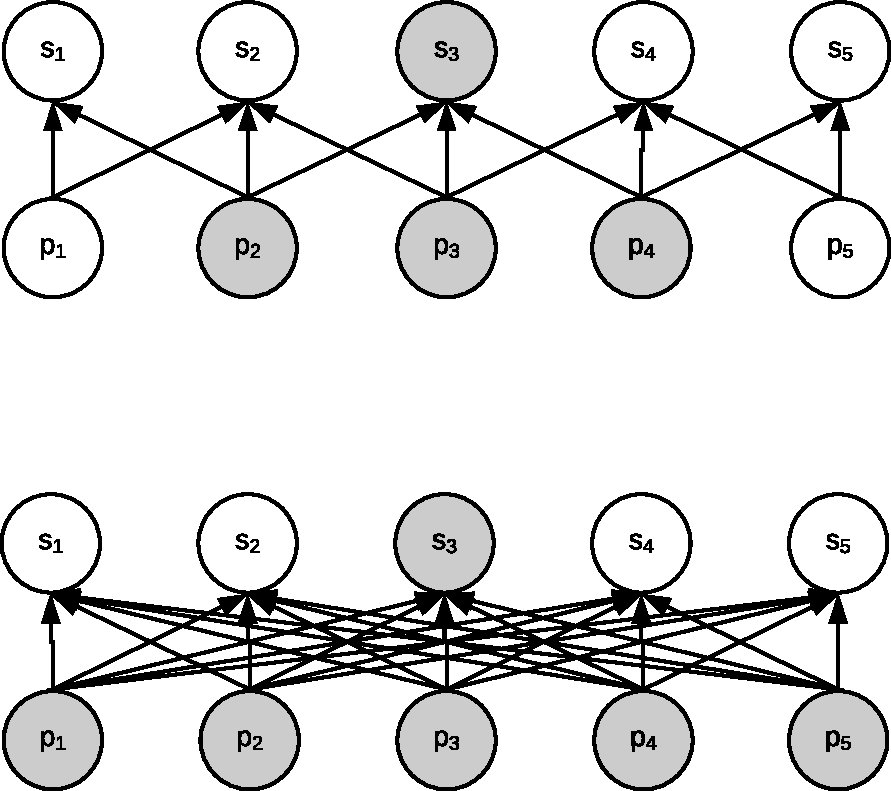
\includegraphics[width=.6\textwidth]{obrazky-figures/sparse_a.pdf}
    \caption{\textit{Sparse interaction viewed from above}: Highlighted portion of the image shows all units affecting the current layer ($s$ units). The amount of units is smaller on the top picture. That represents sparse interaction. On the bottom is the same situation, when the current layer is formed by matrix multiplication in a traditional network.}\label{fig:sparse_a}
\end{figure}

However, this view limits us just to direct influence on a unit. Receptive field lists also indirect influence, hence when multiple convolutional layers are used by the network the field grows. This can be seen on figure\,\ref{fig:receptive}. The effect can be enhanced when network contains additional features like \textit{strided convolution}\,\ref{ss:strided} or \textit{pooling}\,\ref{ss:pooling}. This means, despite the direct influence is very sparse, the final impact through indirect influence can make the units deeper in the network connected to most of the image on input.

\begin{figure}[ht]
    \centering
    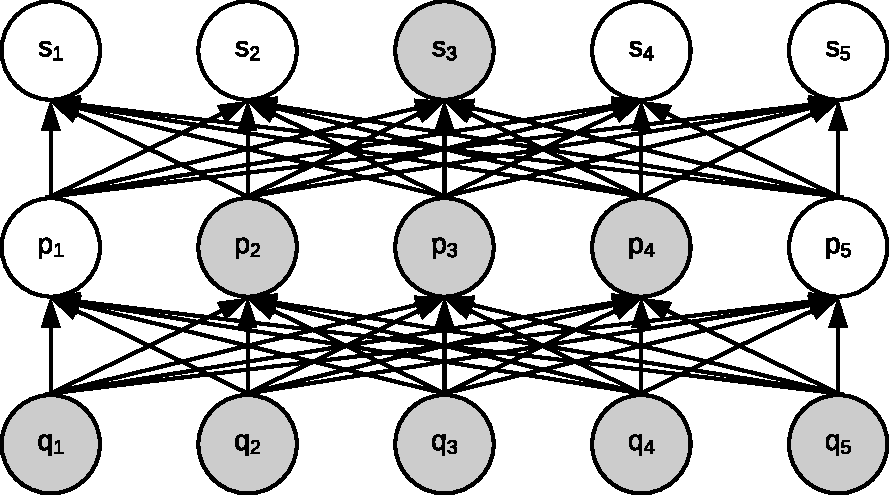
\includegraphics[width=.6\textwidth]{obrazky-figures/receptive.pdf}
    \caption{Receptive field of unit $s_3$}\label{fig:receptive}
\end{figure}

\subsubsection{Parameter sharing}

A feature of convolution referring to a reuse of parameters in more than one computation. In matrix multiplication, each weight element is calculated and used only once when computing the output. The weight is multiplied by one element of the input and then never used again. In contrast, convolution keeps it is kernel the same an uses its elements for every output calculation. This brings an advantage of learning just one set of weights for the whole input, rather than computing and remembering a set of weights for each output unit. Parameter sharing has no impact on forward propagation but it does further improve memory efficiency of a stored model.

\subsubsection{Equivariant representation}

A function is equivariant to another when $f(g(x)) = g(f(x))$. Convolution is naturally equivariant for example to translation\,\cite[p.~339]{deeplearningbook} . Imagine we have an input image and we shift the image some pixels to any direction of choice. When convolution is performed, the same kernel is applied to any set of pixels, therefore the set of features, our network layer aims to collect, can be found in the shifted image as well as in the original. It would just appear shifted in the output feature map. Here we can benefit from parameter sharing in use cases like edge detection. We're interested in the same feature, no matter where it appears on the image. In other use cases, like for example face detection, we might not be interested in the full parameter sharing. Imagine we have a kernel which is trained to detect a mouth. In order to work properly, we should restrict this kernel to look for the feature only in bottom portion of the picture, because detecting a mouth on forehead would not result in proper outputs. We'll cover more about multi-kernel convolution layers later.

\subsubsection{Variable size of the input}

Convolution can process data samples of different sizes. When the use case requires the network to be robust enough to properly process for example images, where each of the sample has different dimensions, this is a problem in matrix multiplication. The network can't apply the fixed size weight matrix on an input of different size. On the other hand, convolution is easy to perform, the situation is really similar to input of a fixed size, just the kernel is applied different amount of times.

\subsection{Pooling}
\label{ss:pooling}

In neural networks, convolution layer does not mean solely a convolution operation is applied\,\cite{handbook_face}. Typically such layer consists of multiple stages:

\begin{enumerate}
    \item \textbf{Convolution stage}: Multiple parallel convolutions are computed, which produces a set of linear activations.
    \item \textbf{Detector stage}: Each of the linear activations from previous stage is run through a nonlinear activation function.
    \item \textbf{Pooling stage}: Further modification of the layer.
\end{enumerate}

The last, pooling stage, provides better understanding of the convolution output. Instead of returning a set of features, it reduces redundancy of neighbouring outputs and provides a summary statistics. This helps the network to be invariant to small transition of the input. This means that if we translate the input of small amount of pixels, the output stays the same. This makes such network more robust. In a situations like a face detection, we don't need to know exact pixel coordinates of a feature, of an eye for example. We just need to define a region, where we are looking for such feature.

There are many pooling operations, let's list some of the most popular ones like \textbf{max pooling}\,\cite{maxpooling} (reports the maximum output in rectangular neighbourhood), average of rectangular neighbourhood, $L^2$ norm of the rectangular neighbourhood, and weighted average of distance from the central pixel.

Invariance to transition is produced by pooling over spatial regions, however pooling layer can learn an invariance to a transformation of other kinds as well. That happens if we pool over outputs of other separately parametrized convolutions. As an example you can see an invariance to slant in cursive on figure\,\ref{fig:pooling}. This principle is accented mainly in max-out networks\,\cite{maxout}.

\begin{figure}[ht]
    \centering
    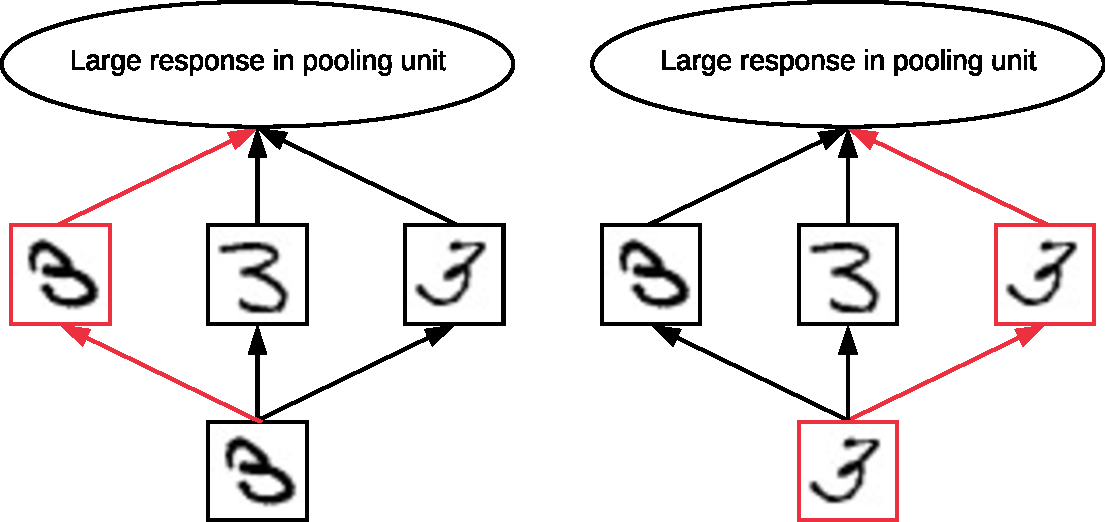
\includegraphics[width=.8\textwidth]{obrazky-figures/pooling.pdf}
    \caption{\textit{Pooling response with learned invariance to slant}: Here we have 3 filters, where all of them had a task to learn a handwritten number 3. Each of them resulted in learning of different slant of the number. When a number 3 is given as the input, one of the filters will match it and cause a high activation in corresponding detector unit. Due to use of pooling, the max pooling unit has a large activation as well, no matter which filter matched the number.}\label{fig:pooling}
\end{figure}

Since pooling can summarise a response of layer over whole neighbourhood of input units, it is not necessary to have the same amount of pooling units as the detectors. We can leverage pooling to provide down-sampling as can be seen in figure\,\ref{fig:downsample}. That further improves performance of the network since it lowers the amount of inputs for the next layer.

\textbf{Pooling with down-sampling} is an essential step when dealing with input of variable size. Let's say we want to use the convolution to detect a face on images with different resolutions. We have learned our detectors to register mouth in the bottom half of the image and another two sets of detectors to locate eyes, each in one of the top quadrants. We can use convolution layer with down-sampling pooling to provide the required classification. We expect to be provided by 3 activations on the output, and each of the detector has assigned its portion of the input. It does not matter, if the portion contains one amount of pixels or much more.

\begin{figure}[ht]
    \centering
    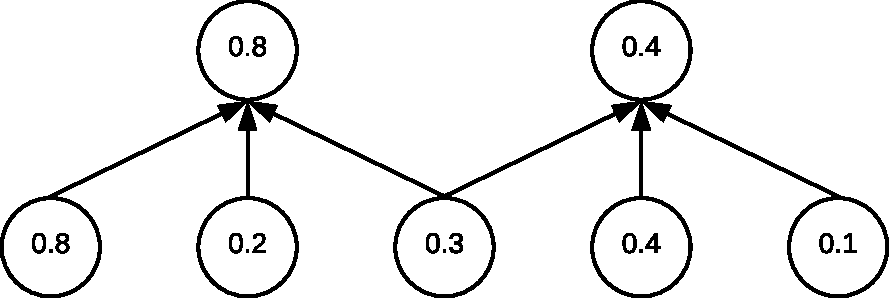
\includegraphics[width=.6\textwidth]{obrazky-figures/downsampling.pdf}
    \caption{Pooling with down-sampling}\label{fig:downsample}
\end{figure}

In deep learning this is often the case. We don't refer to convolution as a simple single operation as described in the beginning of this chapter. Such convolution layer with a single kernel would be capable of extracting only a single feature, although in many spatial locations. Usually many convolutions are applied and performed in parallel. That can provide many different kernels for different features, which are interesting for the use case. As a result, the network can locate many kinds of features at many locations.

\subsection{Strided convolution}
\label{ss:strided}

Also when we have stumbled upon the down-sampling in pooling, this step can be sometimes omitted and simplified even more. Although the result is similar to the pooling with down-sampling, the logic in based on different assumptions. In pooling operation, we leverage all the information retrieved by the convolutions and simplify the output.

A strided convolution is rather avoiding some of the convolutions at all. That further lowers the computational costs, hence at a risk of not extracting all the features in such detail. In this case we sample pixels in every direction with a step of $s$. The step $s$ is called a \textbf{stride}. It is also possible to define a separate stride for each step direction.

\begin{figure}
    \centering
    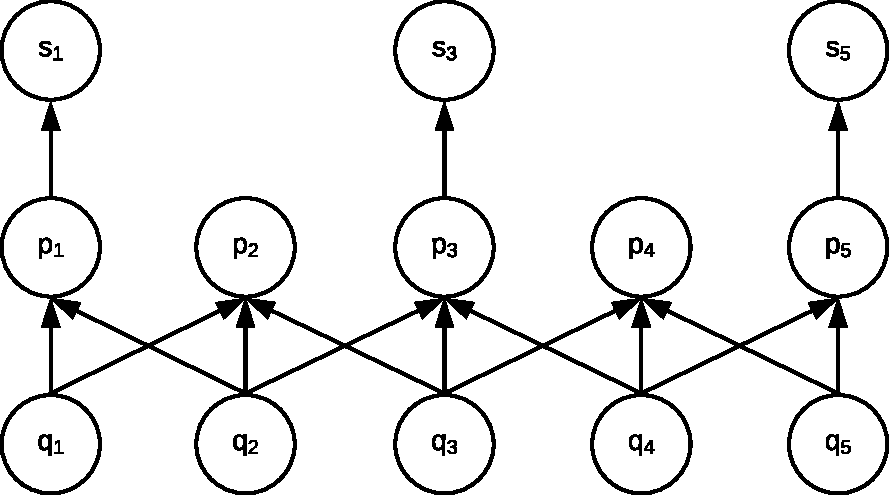
\includegraphics[width=.6\textwidth]{obrazky-figures/conv_down.pdf}
    \caption{Convolution and pooling with down-sampling}\label{fig:conv_down}
\end{figure}


\begin{figure}
    \centering
    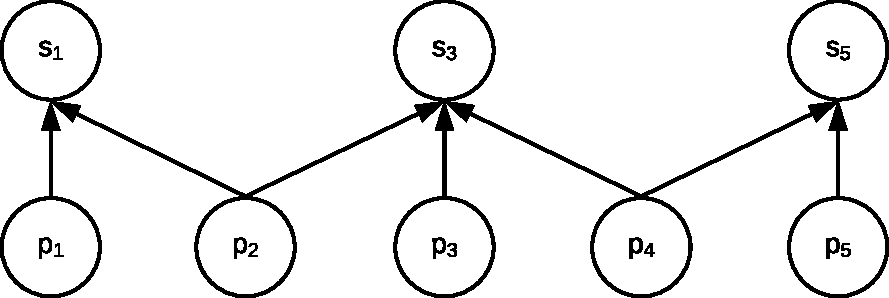
\includegraphics[width=.6\textwidth]{obrazky-figures/strided.pdf}
    \caption{Strided convolution}\label{fig:strided}
\end{figure}

As it can be clearly seen on the images\,\ref{fig:conv_down} and\,\ref{fig:strided} the two step down-sampling is computationally more expensive than the strided optimisation, while it can provide similar results.

\subsection{Zero padding}

Another feature which is essential to CNNs implementation is padding with zeros. This maintains the network's ability to preserve the width of its input if needed. The input tensor is padded with zeros on the ends, so a convolution operation does not shrink the size of input vector by a fraction of kernel. Without padding we are forced to either keep kernels small, or let the networks shrink in spatial extent. Both are extreme limitations of network's power. Padding allows to control independently both: the size of kernel and resolution of the output.

\subsection{Other convolution layer types}

Sometimes our desire is to rather use locally connected layers. This resembles a discrete convolution with small kernel, but without parameter sharing. Therefore this layer type is sometimes called \textbf{unshared convolution}\,\cite{locally_connected}. Unshared type of convolutional layer is useful when we aim to detect features, which are local and there's no assumption that the same feature should occur across all the input.

Another type available is a \textbf{tiled convolution}\,\cite{tiled_conv} layer. A layer type meant to offer a compromise between locally connected layers and convolutional layers. Instead of learning a set of weights for every spatial location, this layer type provides tiling. That means a single set of weights is learned and it is later applied in rotation, providing different set of weighs for neighbouring locations. This makes the outcome similar to locally connected layer, while keeping the benefit of lower cost of convolutional layer, since requirements to store parameters would grow by factor of kernel set size, instead of size of a whole feature map. A comparison overview of different convolution layer types can be seen on figure\,\ref{fig:compare_layers}.

\begin{figure}
    \centering
    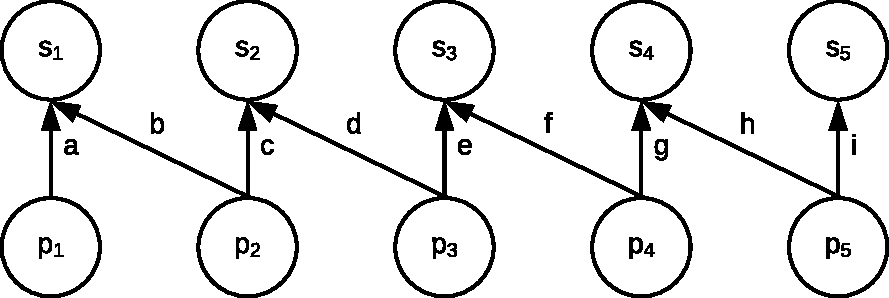
\includegraphics[width=.6\textwidth]{obrazky-figures/locally_connected.pdf} \\
    Locally connected \\
    \bigskip
    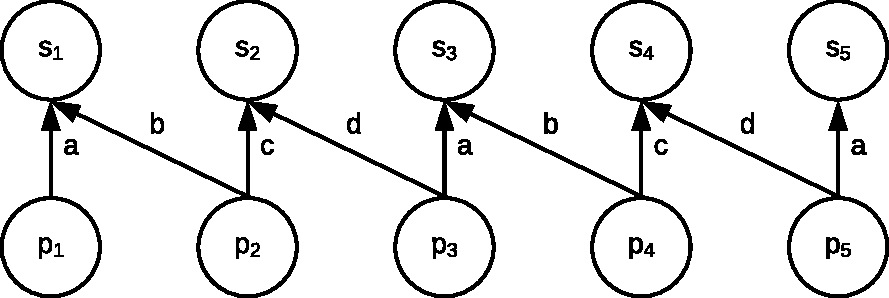
\includegraphics[width=.6\textwidth]{obrazky-figures/convolution_tiled.pdf} \\
    Tiled convolution \\
    \bigskip
    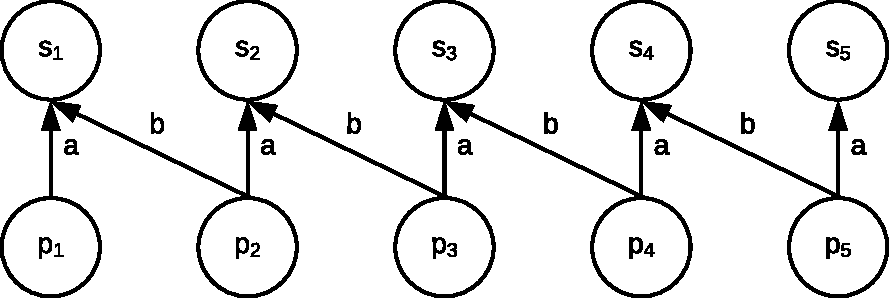
\includegraphics[width=.6\textwidth]{obrazky-figures/convolution_std.pdf} \\
    Standard convolution \\
    \bigskip
    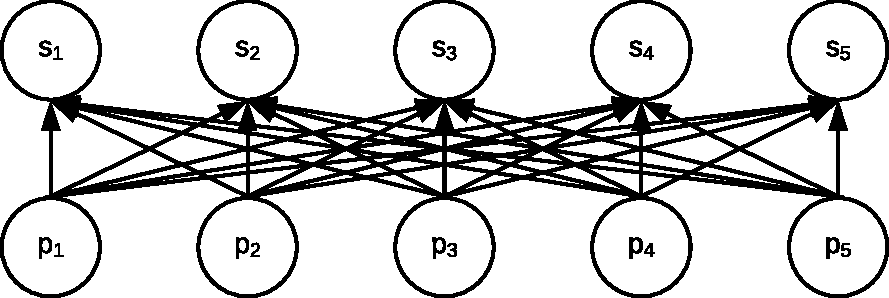
\includegraphics[width=.6\textwidth]{obrazky-figures/fully_connected.pdf} \\
    Fully connected \\
    \bigskip
    \caption{Comparison of convolutional layers}
    \label{fig:compare_layers}
\end{figure}

\section{Capsule neural networks}

Convolutional neural networks are a state-of-the-art of current deep learning. They are hugely popular and they can provide great results and solve problems, which were unimaginable before. Despite all their power they embody fundamental drawbacks and limitations\,\cite{capsule_compare}. This and availability of grater computational power lead to creation of Capsule neural networks (CapsNET)\,\cite{capsule}.

\subsection{Rationale}

CNNs operate with features and their recognition. Deeper convolution layer detect simple features, for example edges or colour gradients. Layers higher in the network are designed to detect specific combinations of such features and creates more complex ones. And finally, on the very top of the network, a dense layer takes the very high level features and provides a prediction of classification. And since many times the convolution is made invariant to different transformations, this can lead to impossible results. Mere presence of an object provides indication of feature presence. Relation between detected features is not considered at all. When simple features are composed to a more complex ones, translational or rotational relationship does not play any role.

We have already tackled the way CNN is using to deal with this problem. Pooling and more convolutional layers of smaller kernels are applied to reduce spatial size of information lost during each convolution. This aims to increase the field of view for convolutional layers higher in the network, therefore allowing them to locate features in larger portion of the input image. Pooling made CNNs surprisingly effective and one of the top performing architectures, though still enhancing loss of information.

Prof. Geoffrey Hinton, one of fathers of deep learning and praised founder of many principles and author of algorithms, is also the author of capsule neural networks. Hinton wrote\,\footnote{\url{https://www.reddit.com/r/MachineLearning/comments/2lmo0l/ama_geoffrey_hinton/clyj4jv/}}:
\begin{quotation}
    The pooling operation used in convolutional neural networks is a big mistake and the fact that it works so well is a disaster.
\end{quotation}

To demonstrate this drawback imagine a CNN face detector. Deeper layers of network detects parts of facial features. The higher layers combine these parts into complex features like an \textit{eye}, \textit{nose} or \textit{mouth}. Our multi-kernel convolution would allow us to define regions, where we expect such features, though we can't define the relation between them. The network can simply recognise an image as a valid face, despite for example the \textit{eye} is rotated to the opposite direction than a \textit{mouth}. An extreme demonstration of such problem can be seen on figure\,\ref{fig:capsule_face}.

\begin{figure}[ht]
    \centering
    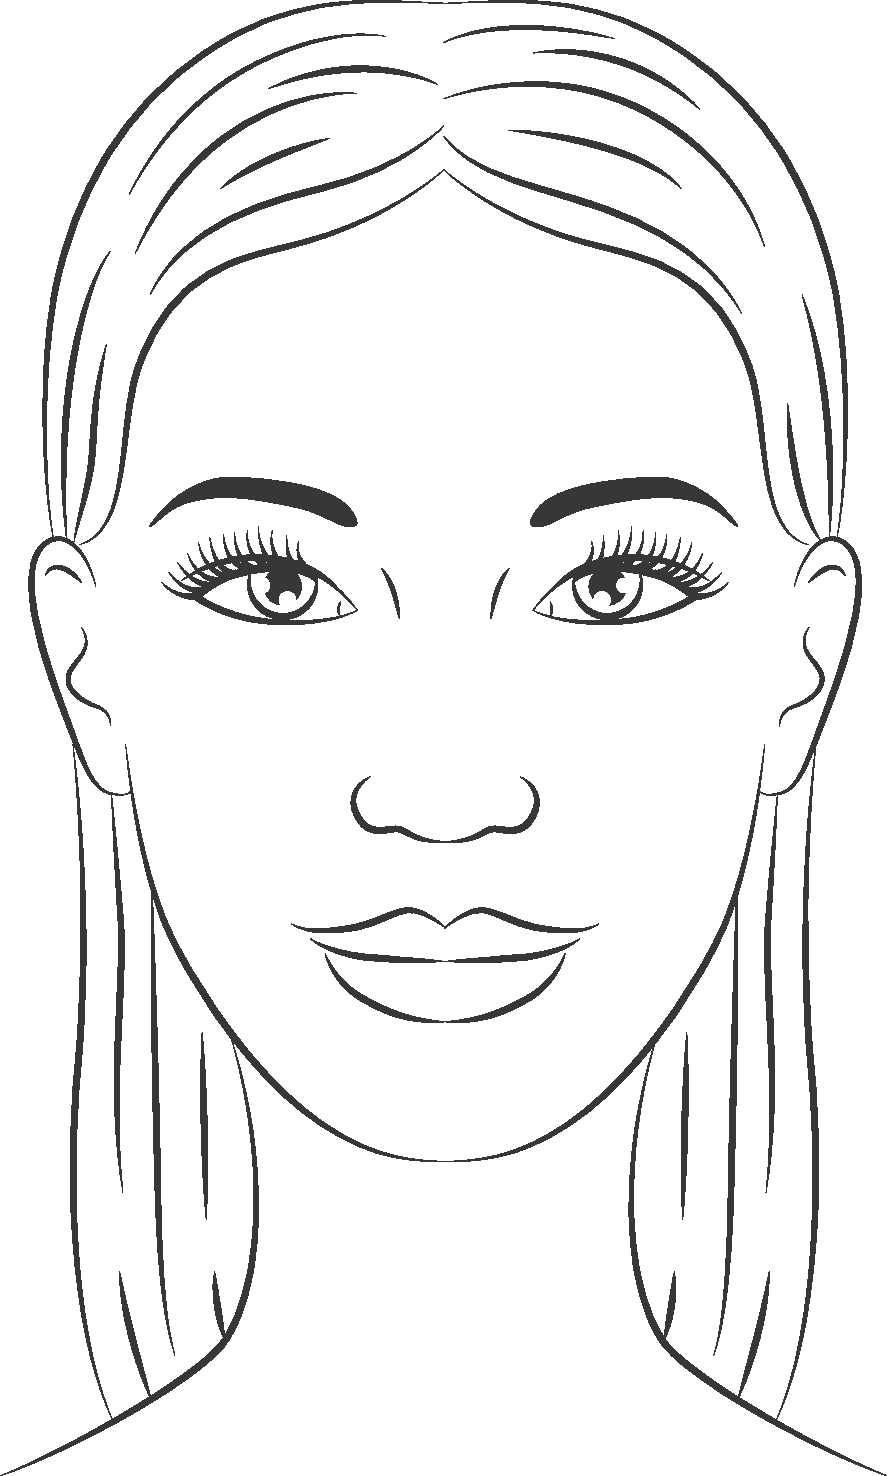
\includegraphics[height=0.3\textwidth]{obrazky-figures/face_normal.pdf}
    \hspace{10em}
    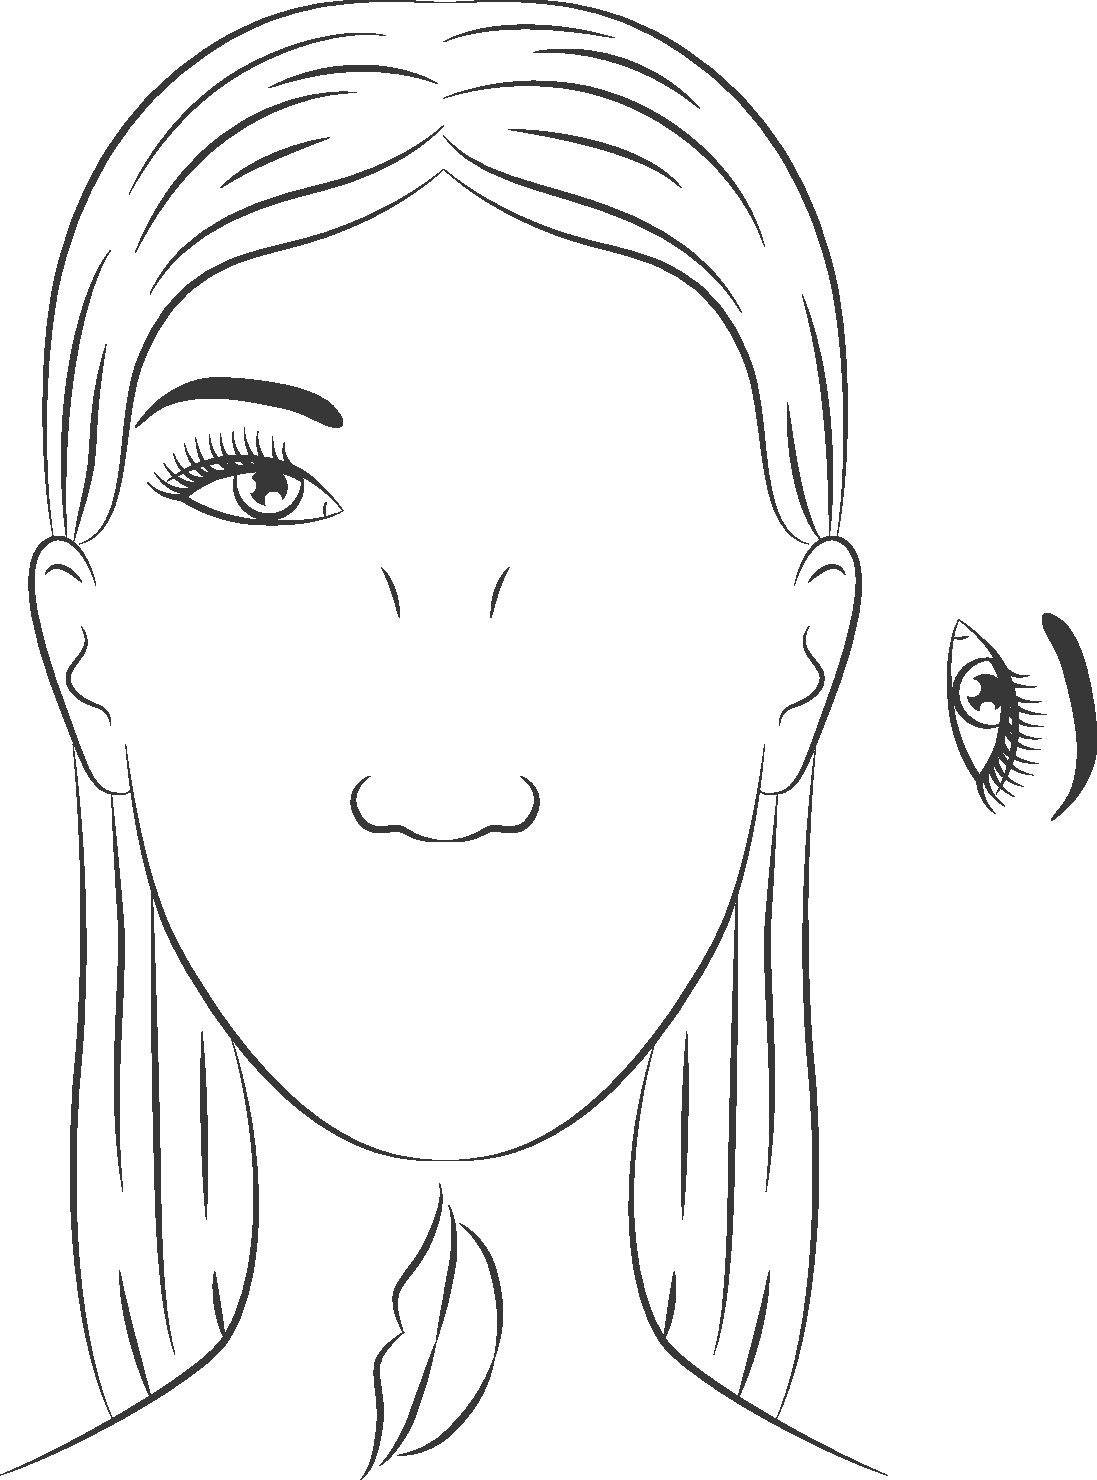
\includegraphics[height=0.3\textwidth]{obrazky-figures/face_disorted.pdf}
    \caption{Both of these images can be evaluated to be a face. Spatial location, relation and pose between simpler features are not considered by this type of network. Both images appear similar to CNN. \textit{Original artwork provided by Freepik\,\cite{freepik}}}
    \label{fig:capsule_face}
\end{figure}

\subsection{Inverse graphics}

Hinton, inspired by computer graphics, tried to explain and reconstruct human brain's visual cognitive functions. The brain itself in fact does the opposite process to \textit{rendering} we know from computer graphics. Hinton calls it \textbf{inverse graphics}. A visual information is decomposed into a hierarchical representation of objects, which are matched against known, learned patterns. This relationship matrix is stored in our brains. One key factor is that object representation is not dependent on view angle.

So how do we model this hierarchical relationship inside a neural network? Here we can learn from solutions already discovered in another field -- in computer graphics. 3D modelling uses something called a \textbf{pose}. This represents relation between 3D objects and provides a rotation and translation transformation matrix. In neural networks we represent that as a 4D \textit{pose matrix}\,\cite{capsule}. This results in combination of information about object relations with internal representation of object data. Hence it becomes easy for a model to recognise that it just sees a different view of something it already saw before.

\begin{figure}[ht]
    \centering
    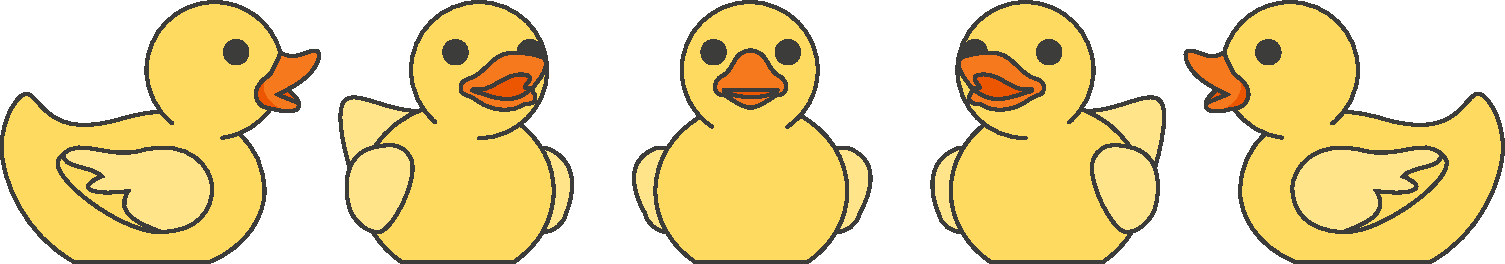
\includegraphics[width=.8\textwidth]{obrazky-figures/duck.pdf}
    \caption{CNN struggles to recognise this is the same object. Human brain, on the other hand, immediately understands that objects on the picture are identical, despite being viewed from multiple different angles. \textit{Original artwork provided by Freepik\,\cite{freepik}}}
    \label{fig:duck}
\end{figure}

Let's discuss a situation on the figure\,\ref{fig:duck}. A human looking at this picture can easily recognise, it is a rubber duck viewed from different angles. Our internal representation of a rubber duck is independent on the viewing angle. It may be the first time that these particular pictures are shown to you, although you simply know their meaning. Since there's no internal representation of 3D space in CNNs, it really struggles. On the other hand, for CapsNET, this problem is pretty easy, since the 3D relations are explicitly modelled. Experiments shown that usage of capsule neural networks can further reduce the error rate\,\cite{capsule_compare}.

And this is not the only benefit of usage of capsules. It also significantly lowers the amount of data required to train such network to achieve comparable performance to a CNN. And this make sense, since capsule theory is much closer to the way how brain does work. If a brain tries to learn to distinguish a horse from a cow, it only needs to be presented with few images, at most couple of dozens. CNN would require to be presented by many thousands of image samples, to achieve comparable performance. In this particular aspect we can compare CNNs to a brute-force approach to deep learning.

\subsection{Understanding capsules}

Let's step back and introduce capsules in the CapsNet networks. What does a term \textit{capsule} actually mean? What is the mathematic representation and what key principles are used? How we can represent it as a neural network architecture? How does a network using capsules look like from the engineering aspect? And how should such network look like in our particular use case?

There are many ways to implement capsules and in this example we will follow Hinton\,\cite{capsule} and use a simple, 3 layer shallow capsule network with dynamic routing. As shown later, such shallow network and straightforward implementation works well when used together with dynamic routing and can achieve results comparable to much deeper CNN networks.

Desired representation of a capsule layer output in CapsNet network represents a probabilistic likelihood of the entity mapped by one particular capsule being present in the current input. To facilitate this we use a non-linear activation called \textbf{squash}\ and is shown as equation \ref{eq:squash}. It ensures that the length of a vector is converted into a probability score of feature presence in current input kernel for each capsule. The aim is to resize vector based on their size. Shorter vectors get shrunk to minimal lengths while long vector are shrunk to size slightly below 1. This non-linearity can be later leveraged in discriminative learning process.

\begin{equation}
    v_j = \frac{\norm{s_j}^2}{1 + \norm{s_j}^2} \frac{s_j}{\norm{s_j}}
    \label{eq:squash}
\end{equation}

In this equation a squash activation is computed for a capsule $j$ where $v_j$ would represent squashed output and $s_j$ is the total input.

In any later layer except the first layer of capsules the capsule can understand the $s_j$ input as a weighted sum mapping over all prediction vectors $\hat{u_j|i}$ decided by the capsule layer below. This prediction vectors are a product of $u_i$ output of previous capsule layer and its $W_{ij}$ weights matrix.

\begin{equation}
    s_j = \sum_{i}c_{ij}\hat{u}_{j|i},\quad \hat{u}_{j|i} = W_{ij}u_i
    \label{eq:capsule}
\end{equation}

Here we are introducing $c_{ij}$ coupling coefficients which are determined by the dynamic routing process in multiple iterations. The $c_{ij}$ coefficients are computed for each capsule $i$ in relation to every capsule $j$ in the layer above. For each capsule $i$ the sum of these coefficients is equal to 1 and represents a special soft-max for routing. This activation uses initial logits $b_{ij}$ that are log prior probabilities of the likelihood a capsule $i$ is coupled to capsule $j$. In general, routing provides each capsule $j$ a mean to determine which capsules $i$ are interesting enough and aligned in the same fashion for it to base its prediction upon. This coupling is determined independently on current input.

\begin{equation}
    c_{ij} = \frac{exp(b_{ij})}{\sum_{k}exp(b_{ik})}
    \label{eq:softmax}
\end{equation}

Later on we will define two distinct layer types: \textit{prediction capsules} and \textit{primary capsules}. These are required to communicate and rate the activations based on accuracy of the prediction. The algorithm used is called \textbf{dynamic routing by agreement} and is described in greater detail by Hinton in publication \textit{Dynamic routing between capsules}\,\cite{capsule}. It utilizes the already described coupling coefficients and log prior. The algorithm goes as this:

\begin{algorithm}[H]
    \caption{Dynamic routing by agreement}\label{alg:routing}
    \begin{algorithmic}[1]
        \Procedure{ROUTING}{$\hat{u}_{j|i}, r, l$}
        \ForAll{capsule $i$ in layer $j$ and capsule $j$ in layer $(l + 1)$} $b_{ij}\gets 0$ \EndFor
        \For{$r$ iterations}
            \ForAll{capsule $i$ in layer $l$} $c_{i}\gets softmax(b_i)$ \EndFor
            \ForAll{capsule $j$ in layer $(l + 1)$} $s_{j}\gets \sum_ic_{ij}\hat{u}_{j|i}$ \EndFor
            \ForAll{capsule $j$ in layer $(l + 1)$} $v_{j}\gets squash(s_j)$ \EndFor
            \ForAll{capsule $i$ in layer $l$ and capsule $j$ in layer $(l + 1)$} $b_{ij}\gets b_{ij} + \hat{u}_{j|i} v_j$ \EndFor
        \EndFor
        \State \textbf{return} $v_j$
    \EndProcedure
    \end{algorithmic}
\end{algorithm}

The aim is simple, yet harder to achieve. All and every capsule in \textit{primary capsule} and \textit{prediction capsule} layers are made to agree on the location of the features in space and their orientation. At first all the routing logits $b_{ij}$ are initialized to zero. That means each input capsule's output is sent to the next layer's capsules with equal probability $c_{ij}$. In time the logits are learned and since they are independent on the current image\footnote{Each image is expected to include one and just one face, not more.}, they can be trained at the same time as all the other weights. Their only dependency is the type and location of the capsules involved. Its training process involves iteratively adjusting and refining the logits based on measurement of agreement between the prediction $\hat{u}_{j|i}$ made by capsule $i$ in the underlying layer and current output $v_j$ of each capsule $j$ in the layer above.

\begin{equation}
    a_{ij} = v_j \cdot \hat{u}_{j|i}
    \label{eq:agreement}
\end{equation}

The measuring of agreement is simplified to a scalar product as per equation\,\ref{eq:agreement}. This rate is used to as an addend to the log prior $b_{ij}$ and used to compute new value of the coupling coefficient $c_{ij}$.


\subsection{Architecture using capsules}

Before we move on and utilize this principles, we need to step back and understand the capsule networks as whole. Generally speaking a Capsule network (CapsNET) consists of two parts where each has a distinct use: \textbf{Encoder} and \textbf{Decoder}:

A decoder network is a fully connected (dense) or convolutional network, which purpose is simply to reconstruct an image based on prediction. This is used to provide proper feature adaptive learning experience in order to maximize classification potential of the encoder, in other words its a regularization method for capsule networks to reach valid conclusions. Based on recognized features and selected activation in the encoder, decoder attempts to recreate the input object. In simple use cases like MNIST classification a 3 layer dense network can be used. This was demonstrated by Hinton and can be seen on figure\,\ref{fig:decoder}. In more feature rich environment with bigger resolution required on input a fully connected layer doesn't provide enough interpolation and resizing capabilities so a convolutional network with resize (enlarge) has to be used. Such network can be of up to 10 layers total. In later chapter we will provide examples of such decoder networks.

\begin{figure}[ht]
    \centering
    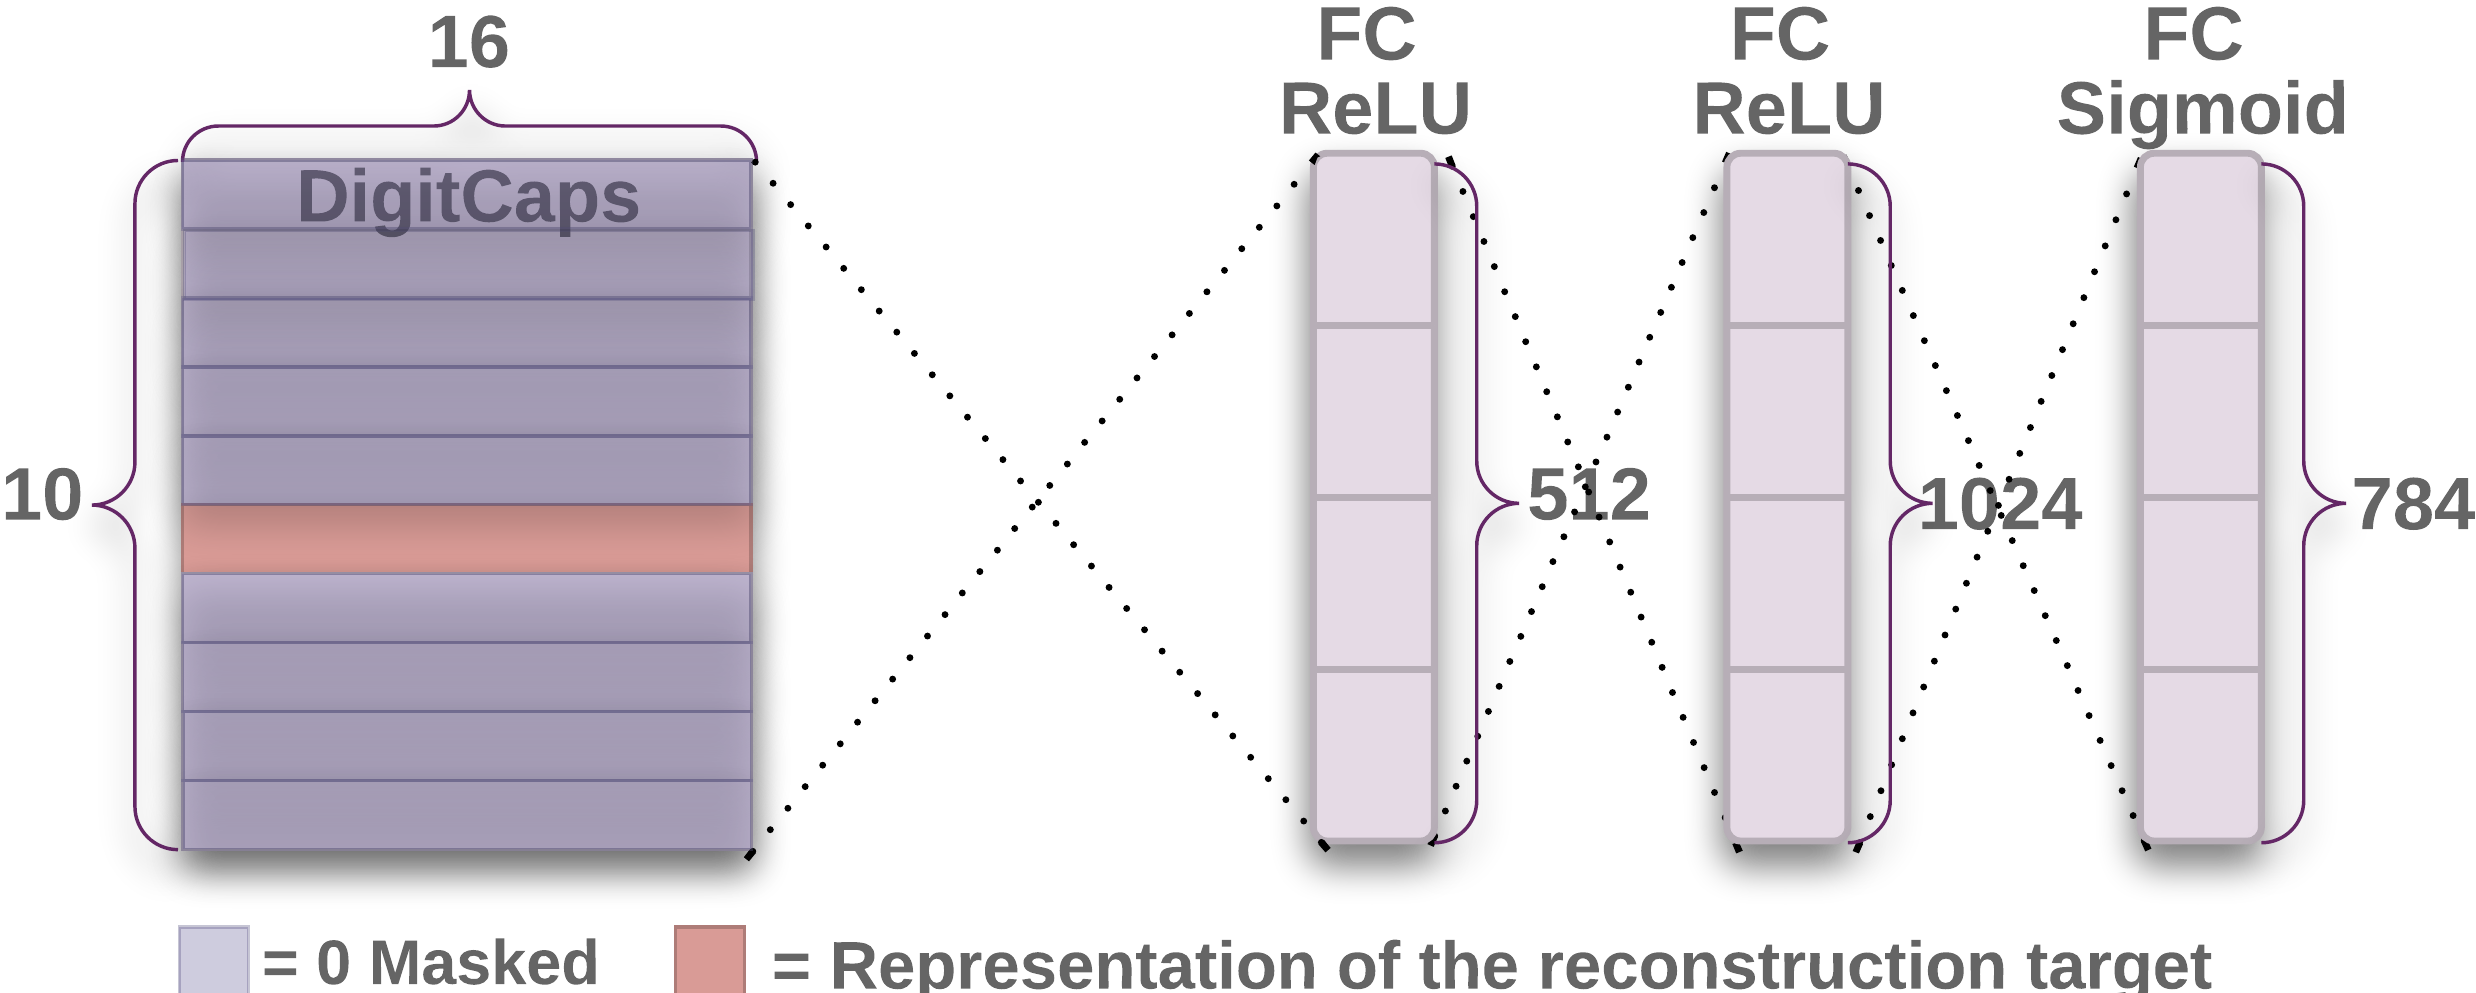
\includegraphics[height=11em]{obrazky-figures/reconsArch.png}
    \caption{Decoder architecture as per Hinton\,\cite{capsule}}
    \label{fig:decoder}
\end{figure}

Encoder is simply the gro of capsule network. This is the truly capsulized network. There are many configurations available, though with growing complexity\,--\,meaning adding capsule layers, the computational complexity grows exponentially. This is due to routing and amount of connections required between each capsule. In this thesis, we will be using the Hinton's hinted layering with a slight twist to facilitate more detailed and granular feature recognition across much wider space.

As said the 3 layer encoder consist of two convolutional layers (one traditional, one capsule-based) and one capsule-based fully connected layer. The first layer
\textit{encoder\_conv1} is a traditional 2D convolution. Each pixel intensity of the input image gets converted in this layer to the activation in a detector of local features. Detected local features are used as input for next layer, primary capsules.

\begin{figure}[ht]
    \centering
    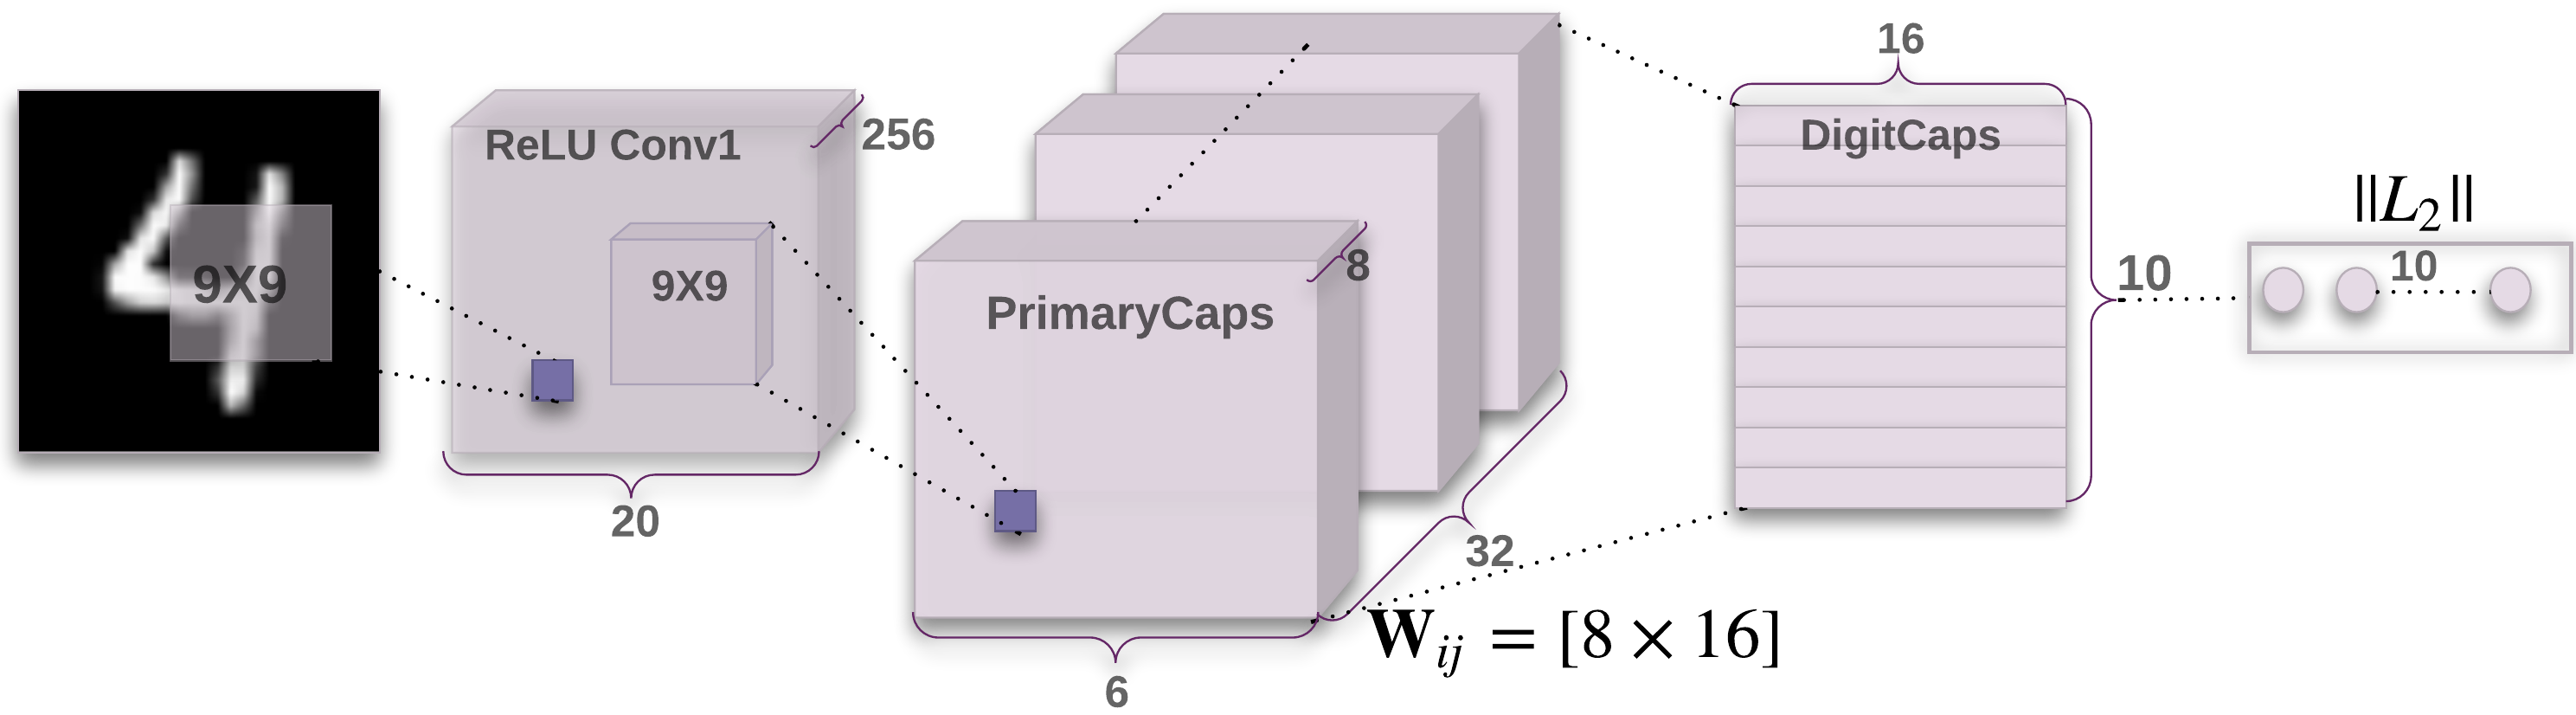
\includegraphics[width=\textwidth]{obrazky-figures/capsulearch.png}
    \caption{Encoder architecture as per Hinton\,\cite{capsule}}
    \label{fig:encoder}
\end{figure}

Naturally each of these parts of the network can be assigned their own loss function. A different balance\,--\,loss weight enforced over each of these functions can greatly improve the overall loss of the network. For \textit{decoder} a loss function would be straightforward to guess. Since we're dealing with images, 2D data comparison, for example a simple \textit{mean squared error} is a suitable metric.

\begin{equation}
    MSE = \frac{1}{n} \sum_{i=0}^{n} (Y_{i} - \hat{Y}_{i})^2
\end{equation}

On the other hand, the encoder part required more sophisticated mean to compute its inconsistency between the predicted value and its ground truth. Therefore a \textit{margin loss} is used for each label in which we're classifying the images. For each of them and individual loss is calculated and the total loss is said to be a simple sum of these partial losses:

\begin{equation}
    L_k = T_k max(0, m^+ - \norm{v_k})^2 + \lambda (1 - T_k) max(0, \norm{v_k} - m^-)^2
    \label{eq:margin_loss}
\end{equation}

where, $T_k = 1$ is a hot one encoded truth of the capsule belonging to that particular label. Then $m^+ = 0.9$ and $m^- = 0.1$ are the loss boundaries and we use the down-weighting factor of $\lambda = 0.5$ to stop shrinking in lengths of activation vectors when initial learning happens\,\cite{capsule}.

\subsection{Primary capsules}

This composite layer encapsulates a convolution with vectorization and \textit{squashing}. Therefore this layer is also called \textit{convolutional capsule layer}. It provides knowledge about greater context of each local feature, and makes more abstract detection about overall shape and orientation of such feature. Key factor in this layer is a non-linear activation called \textit{squashing}. We've already covered the squashing function by equation\,\ref{eq:squash}. Hinton, describes this layer\,\cite{capsule} as:

\begin{quotation}
    In convolutional capsule layers each unit in a capsule is a convolutional unit. Therefore, each capsule will output a grid of vectors rather than a single output vector.
\end{quotation}

The quoted statement stipulates boundaries by which this layer is different to a standard convolution. Since we're not interested in a scalar feature identity, and require more complex result, a whole vector of attributes that holds much broader context of the feature location. This brings couple of limitations of the convolution itself though. For example a strided convolution or pooling would mean disaster for the spatial collocation of a feature. Therefore we eliminate our use of these advanced convolutional optimizations and we are obliged to use a convolution in its most simple and pure form.

\subsection{Prediction capsules}

Next layer is understood to be a fully connected capsule layer, which purpose is to rate the features located by the previous \textit{primary capsule} layer and bundle the smallest amount of unique activation per label. As it may sound confusing, we need to elaborate further and step by step. We already know, that the output of previous layer in each of its capsules is a local grid of vectors which are unique to each its member as well as for each capsule. Key word is "grid". It signifies the output is three dimensional. However traditionally a feature is understood as a 2D location. Our primary capsules holds also another interesting factor to this. We can now understand and recognize a feature in relation to others. And that's precisely what is done in this layer. The amount of prediction capsules corresponds to the amount of target labels. Therefore each capsule is mapped to one particular label, in our case an identity, and is expected to locate the features which are unique to this particular identity as well as all the common features which define a face. However this is not an easy task, and a simple weighted multiplication over a kernel would not provide enough insight into the complicated data. Therefore an algorithm called \textit{dynamic routing} is used. The main purpose is to recognise that particular features which holds the same or similar context as the others for each particular label. The context can be of many different types, from simple distance of multiple features in 3D space, over a consistent angle hold between two features, to for instance a simple contextualized location relative to other features.
